%!TEX root = lec05_query_processing.tex


\begin{frame}

SQL is a \alert{high level declarative language}:
\begin{itemize}[-,noitemsep,topsep=-0.5em]
\item A query specifies \textbf{what} the programmer wants...
\item ... but it does not specify \textbf{how} to compute the answer.
\end{itemize}

\vskip1em

We need to \blue{translate} each SQL query \blue{into} an \blue{an actual executable representation} which the DBMS can process.
\begin{itemize}[-,topsep=-0.5em]
\item Similar to generating executable bytecode from Java.
\end{itemize}

\vskip1em

A \textbf{query plan} is an executable representation of a query.
\begin{itemize}[-,noitemsep,topsep=-0.5em]
\item Query plans, essentially, relational algebra expressions.
\item Recall that we can always translate SQL queries into the algebra because they are equivalent\footnote{Actual implementations of the algebra have operators for advanced SQL features like recursion.}.
\end{itemize}


\end{frame}

%
% --------------------------------------------------------
%

\begin{frame}[fragile]

For example, the SQL query

\begin{center}
\begin{lstlisting}[style=SQL]
SELECT m.director FROM Movie m, Cast c
WHERE m.title=c.title AND m.year=c.year AND
      c.actor='Bill Murray'
\end{lstlisting}
\end{center}

is equivalent to \qquad 
\(\pi_{\texttt{director}} \left(\sigma_{\texttt{actor='Bill Murray'}}
\left(\texttt{\lstinline[style=SQL]{Movie}}\Join\texttt{\lstinline[style=SQL]{Cast}}\right)\right)\)

\vskip2em

\begin{columns}[onlytextwidth]
\begin{column}{0.5\textwidth}
Note that we can represent every algebra expressions as a tree.

\vskip1em

It is common to represent query plans as trees. Most DBMSs have GUIs to let the DBA inspect plans in this way.
\end{column}

\begin{column}{0.5\textwidth}
\begin{center}
\begin{tikzpicture}
    \node (0) at (0,0) {$\pi_{\texttt{director}}$};
    \node (1) [below of=0] {$\sigma_{\texttt{actor='Bill Murray'}}$};
    \node (2) [below of=1] {$\Join$};
    \node (3) [below left of=2] {\lstinline[style=SQL]{Movie}};
    \node (4) [below right of=2] {\lstinline[style=SQL]{Cast}};
    \path[commutative diagrams/.cd, every arrow]
        (4) edge (2)
        (3) edge (2)
        (2) edge (1)
        (1) edge (0);
\end{tikzpicture}
\end{center}
\end{column}
\end{columns}
\end{frame}

%
% --------------------------------------------------------
%

\begin{frame}

The \alert{difference between a plan and an algebra expression} is that the plan specifies \textbf{access methods} are used to read the data and which \textbf{algorithm} is used to implement each operation\footnote{We will see that that are often many choices, especially for joins.}.

\vskip2em

\begin{columns}[onlytextwidth]
\begin{column}{0.5\textwidth}
\begin{center}
\begin{tikzpicture}
    \node (0) at (0,0) {$\pi_{\texttt{director}}$};
    \node (1) [below of=0] {$\sigma_{\texttt{actor='Bill Murray'}}$};
    \node (2) [below of=1] {$\Join$};
    \node (3) [below left of=2] {\lstinline[style=SQL]{Movie}};
    \node (4) [below right of=2] {\lstinline[style=SQL]{Cast}};
    \path[commutative diagrams/.cd, every arrow]
        (4) edge (2)
        (3) edge (2)
        (2) edge (1)
        (1) edge (0);
\end{tikzpicture}
\end{center}
\end{column}

\begin{column}{0.5\textwidth}
\begin{center}
\begin{tikzpicture}
    \node (0) at (0,0) {$\pi_{\texttt{director}}$};
    \node (1) [below of=0] {$\sigma_{\texttt{actor='Bill Murray'}}$};
    \node (2) [below of=1] {\lstinline[style=SQL]{nested_loop_join}};
    \node (3) [below left= 0.35cm and -0.75cm of 2] {\lstinline[style=SQL]{scan(Movie)}};
    \node (4) [below right= 0.35cm and -0.75cm of 2] {\lstinline[style=SQL]{scan(Cast)}};
    \path[commutative diagrams/.cd, every arrow]
        (4) edge (2)
        (3) edge (2)
        (2) edge (1)
        (1) edge (0);
\end{tikzpicture}
\end{center}
\end{column}

\end{columns}

\vskip1em

The \lstinline[style=SQL]{scan()} \textbf{operator} is a full \alert{table scan}, which pulls tuples from a table file (heap or sequential).
\end{frame}

%
% --------------------------------------------------------
%


\begin{frame}{The life cycle of a query}
\begin{tikzpicture}
\node at (0,0) [anchor=south west] {\includegraphics[width=0.75\textwidth]{figures/sample_C_program}};
\coordinate (prepare) at (6.125,4.125);
\coordinate (fetch) at (3.5,2.525);

\only<2-3>\node (compile) [color=fern,draw] at (9.5,5.125) {\begin{minipage}{2.75cm}
\fontsize{8}{9}\selectfont \centering compile SQL query\\
into (algebraic) plan \end{minipage}};
\only<2-3>\draw [->,color=fern] (compile) to[out=270,in=0] (prepare);

\only<3>\node (step) [color=fern,draw] at (9.5,2.65) {\begin{minipage}{2.75cm}
\fontsize{8}{9}\selectfont \centering fetch tuples\\
one-at-a-time \end{minipage}};
\only<3>\draw [->,color=fern] (step) to[out=180,in=45] (fetch);
\end{tikzpicture}
\end{frame}



\begin{frame}

\textbf{Compiling} the SQL query

\begin{center}
\fbox{\clipbox{0pt 110pt 0pt 95pt}{\includegraphics[width=0.75\textwidth]{figures/sample_C_program}}}
\end{center}

\vskip1em

... produces a query plan looking like this:

\vskip1em

\begin{center}
	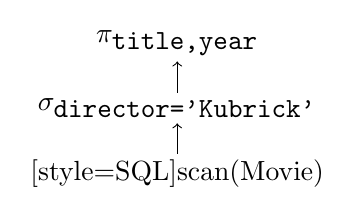
\begin{tikzpicture}[align=center,node distance=0.825cm,every node/.style={inner sep=1,outer sep=1}]
    \node (P1) at (0,0) {$\pi_{\texttt{title,year}}$};
    \node (P2) [below of=P1] {$\sigma_{\texttt{director='Kubrick'}}$};
    \node (P3) [below of=P2] {\lstinline[style=SQL]{scan(Movie)}};
    \path[->] 
    	(P2) edge (P1)
        (P3) edge (P2);
\end{tikzpicture}
\end{center}

\end{frame}



\begin{frame}

The query plan is executed \textbf{iteratively}:

Every call to \lstinline[style=SQL]{sqlite3_step()} fetches \textbf{one \alert{new} tuple} of the answer, and stores it in the heap space of the application.

\vskip1em

\begin{center}
\fbox{\clipbox{0pt 15pt 0pt 150pt}{\includegraphics[width=0.75\textwidth]{figures/sample_C_program}}}
\end{center}

\vskip1em

\lstinline[style=SQL]{sqlite3_step()} has a specific return code to indicate that all tuples in the answer have already been fetched.

\end{frame}

\begin{frame}

\vskip0.75em

\textbf{How is a call to \lstinline[style=SQL]{sqlite3_step()} executed?}

\vskip0.75em

Every node in the query plan implements an interface defining the \lstinline[style=SQL]{getNext()} method, which must returns \alert{a tuple that has not been returned \textbf{by that node} before}.

\vskip1em

\begin{center}
	\begin{tikzpicture}[align=center,node distance=0.825cm,every node/.style={inner sep=1,outer sep=1}]
    \node (P1) at (0,0) {$\pi_{\texttt{title,year}}$};
    \node (P2) [below of=P1] {$\sigma_{\texttt{director='Kubrick'}}$};
    \node (P3) [below of=P2] {\lstinline[style=SQL]{scan(Movie)}};
    \path[->]
    	(P2) edge (P1)
        (P3) edge (P2);

    \pause
    \node (step1) [right=2cm of P1] {\lstinline[style=SQL]{getNext()}};
    \node (app_step) [above of=step1] {\lstinline[style=SQL]{sqlite3_step()}};
    \draw[->,red] ($(app_step)-(0.5,0.175)$) -- ($(step1)-(0.5,-0.175)$);

    \pause
    \node (step2) [below of=step1] {\lstinline[style=SQL]{getNext()}};
    \draw[->,red] ($(step1)-(0.5,0.175)$) -- ($(step2)-(0.5,-0.175)$);

    \pause
    \node (step3) [below of=step2] {\lstinline[style=SQL]{getNext()}};        
    \draw[->,red] ($(step2)-(0.5,0.175)$) -- ($(step3)-(0.5,-0.175)$);

    \pause
    \draw[->,blue] ($(step3)+(0.5,0.175)$) -- ($(step2)+(0.5,-0.175)$);

    \pause
    \draw[->,blue] ($(step2)+(0.5,0.175)$) -- ($(step1)+(0.5,-0.175)$);

    \pause
    \draw[->,blue] ($(step1)+(0.5,0.175)$) -- ($(app_step)+(0.5,-0.175)$);

\end{tikzpicture}
\end{center}

\vskip2em

\lstinline[style=SQL]{sqlite3_step()} calls \lstinline[style=SQL]{getNext()} on the root node of the plan, which leads to further calls to the nodes below, until a new tuple is returned to the application.

\end{frame}


\begin{frame}[fragile]

Those objects returning the ``next tuple'' are called \textbf{iterators}. The DBMS implements at lest one iterator for each kind of operator in the query plan. 

\vskip1em

The DBMS might have different iterators with different algorithms for the same operator. At query optimization time, the DBMS must decide which iterator to use based on the cost of the corresponding algorithm and the available resources.

\vskip1em

Iterators are \textbf{stateful} objects: they cannot return the same tuple more than once, so they need to somehow remember which ones were already returned.
\begin{itemize}[-,topsep=-0.5em]
\item Iterators return \alert{\textbf{\lstinline[style=SQL]{<EOF>}} (end of file)} when there are no more tuples to be returned.
\end{itemize}
 

\end{frame}